\section{Methods}
\subsection{UNet++}
\subsubsection{Motivation}
It's clear that methods before UNet++\cite{unet_pp} can solve general image segmentation problem with decent accuracy, especially when segmenting natural images. However, medical image segmentation require more accuracy in the detail of the segmentation, for example, tumors with ragged edges and more blood vessels on the edge are more likely to be malignant. This puts a higher target for neural networks dedicated to solving medical image segmentation problem, calling for higher-accuracy methods. Also, it's hard for U-Net users to prune U-Net architecture to gain optimal inference time.\\
As a result, two propositions have been made:
\begin{itemize}
    \item Better networks are needed to solve medical image segmentation problems;
    \item Networks need to be more friendly to production situations where recognition speed is vital.
\end{itemize}
In order to meet these requirements, UNet++ was designed above U-Net\cite{unet} with skip connections replaced with dense convolution blocks. We will discuss detailed designs in the next section.

\subsubsection{Detailed Description}
The biggest modification from U-Net into UNet++ was its skip connections. Where were direct skip connections in U-Net was replaced with an array of dense convolutional layers, reforming the network shape as shown in Figure.\ref{fig:unetStructure}.

\begin{figure}[!htpb]
\centering
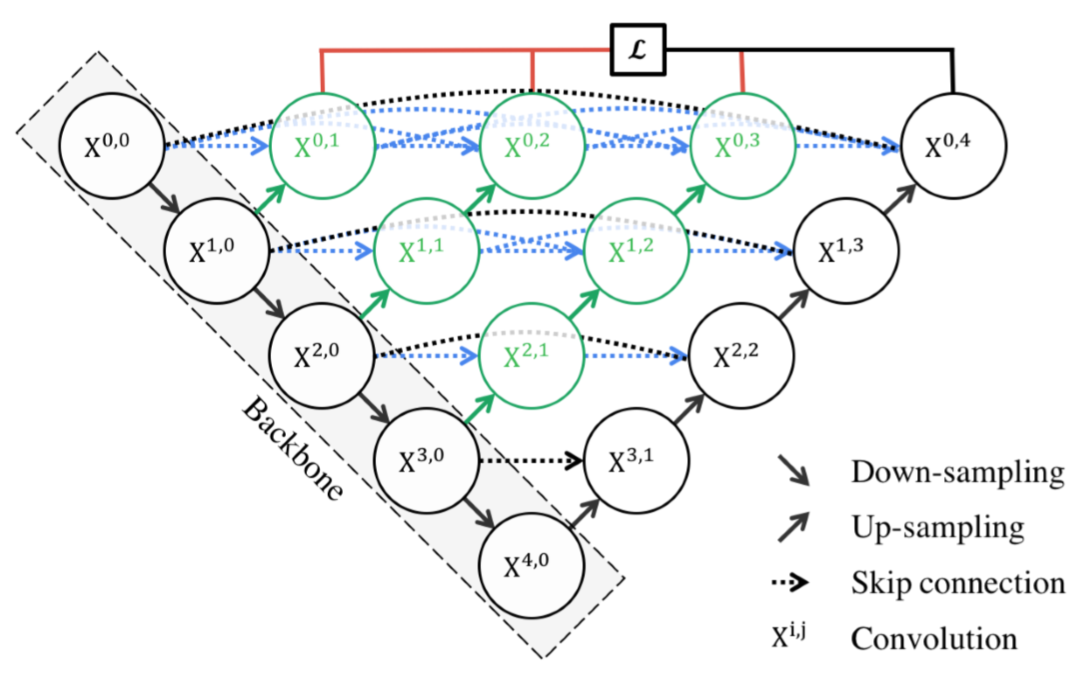
\includegraphics[scale=0.3]{figuras/unetStructure.png}
\caption{Structure of Unet++, where black nodes represent basic U-Net, green nodes are dense convolution layers, blue and green arrows are dense connections and up-sampling, and red connections represent deep supervision.}
\label{fig:unetStructure}
\end{figure}

The basic idea of UNet++ was that, with more dense convolution layers in between, the encoder activation domain would become closer to the decoder network activation domain, thus making finding exact segmentation a easier job. From another perspective, the network structure of UNet++ can be separated into several independent networks, in Figure\ref{fig:unetStructure} there was 4 of them, each having more layers than the last, inheriting the last one's encoder feature map, and adding another layer beyond that. Applying loss at all output positions leverages the popular deep supervision method, not only helping the network to converge better, but also enabling users to prune the network during inference time as users can only use the first several layers of output to determine the result. Consequently, UNet++ with its special dense convolution connections could deal with the two requirements that we mentioned at the same time, thus being more strong and efficiency-aware than bare U-Net.
